\chapter{ Conclusions and Future work }
\label{conclusions}

This work demonstrated an implementation of an electromagnetic transient analysis program using the functional programming paradigm.  At chapter \ref{sec:introduction}, a few questions were proposed. After completing this project, it has become possible to answer some of them or at least suggest a few discussions related to the matter. The upcoming sections bring a summary of this analysis.

\subsubsection{What are the benefits of using a functional programming language? }

For the test case adopted in this work, there were several benefits to this functional approach:

\begin{itemize}
\item During most of the time, when developing the necessary functions,  it was possible to focus on the algorithm, on what the function needs as input data and what it should return as output values. It was not necessary to focus on technical aspects of the language that were not part of the role of the function, such as worrying about vector indexes, clearing temporary values, etc. 
\item There is not a single \lstinline!if/else! block in the Haskell implementation.
\item It was possible to approach the development of functions much more mathematically than programmatically. To compose a new function, it was necessary to determine the input parameters (equivalent to thinking of the \textbf{domain} of the function) and its output (like the \textbf{image} of the function). 
\item Treating software as a mathematical object is a strategy to seek and prove the correctness of the program.
\end{itemize}


\subsubsection{What are the differences to the code base?}


The code base size turned out to be concise - less than 300 lines of code were enough to implement the ETR-P Haskell version. The Matlab ETR-P version has more than 1000 lines of code (it supports more features than the Haskell version, but the number of features is not proportional).

There are many libraries written in Haskell. It is not necessary to write code from zero. There are libraries for web development, machine learning, control systems, matrices and a wide variety of other functions. Most of these libraries are open source and can be found at \cite{hackage}.

Compiling, building and running the project was a straightforward task with Stack \cite{stack}, a cross-platform program for developing Haskell projects. A simple command like \lstinline!stack run! would compile and run the project. The compile process took a few seconds (about 12 seconds).


\subsubsection{What are the technical challenges? }


There is decent support for Haskell at online forums, an essential resource when developing an application. Executing a Google search with an error message usually led to the right answer for the problem. Bleeding-edge technologies and languages may lack this resource. Haskell, on the other hand, is a mature language, and its online knowledge base is broad. Obtaining online information was not a problem. There are also several blog posts, articles from the language maintainers, videos, tutorials and publications in academic conferences.

However, there is a lack of examples for large software applications in the domain of engineering. Most of the material available is restricted to limited, fictional examples (like the ones used in Chapter \ref{haskell} about polygons and shapes). The guides for real-world, large applications are not abundant.

The real technical challenge came during the development of the code. Sometimes, when writing functions, it was difficult to picture them under the ideas of functional programming principles, and the first draft result was very similar to the imperative style, requiring a massive refactoring work to achieve the functional style. Switching paradigms is not a completely obvious task.

Building the appropriate Data Types was also a challenge. Composing information in a structure that maximises not only the readability of the code but that also forms the right algebraic operations required several iterations of code refactoring.

Making the program compile when a  new function was attached was more challenging than finding runtime errors. Most of the times when the program compiled, the output of the program was accurate. Strong and statically typed languages such as Haskell provide a crucial ally for the software engineer - the compiler. In this project, the Haskell compiler caught a vast number of what would have been bugs in runtime execution. This fact confirms the idea that "functional languages are associated with fewer defects than either procedural or scripting languages"\cite{ray2014large}.

\subsubsection{Open source software}

Creating an additional implementation of one of the algorithms to simulate electromagnetic transients that is open source might help future students to understand this approach in practice. They will have access to the code, being able to make changes on it, fix bugs and even implement their own features.   Researches from other institutions can do the same: they will be able to use the code base for their projects, report issues and even contribute to the original project.

Open-source software is an excellent way to show the practical aspects of this work. Feedback from other engineers comes fast and concisely via Github, which also contains an issue tracker (updated to the actual state of this project, check it out at \url{https://github.com/hannelita/thtahs/issues}).

\subsubsection{Notes on building software}

The techniques to build software change from time to time. Not only the technologies but the paradigms,  tools, organisations. Writing code responsibly is more than using bleeding-edge technology. The "Software Engineering Code of Ethics" \cite{gotterbarn1999software} lists a few important principles that should be considered when building programs: "act consistently with the public interest", "managers and leaders shall subscribe to and promote an ethical approach to the management of software development and maintenance", "participate lifelong learning", "ensure their products and related modifications meet the highest professional standards possible". Breaking the monopoly of a single approach is acting ethically when the new projects reach higher standards.

Defining the meaning of "good software" is out of the scope of this work, but certainly, it involves innovation, combining appropriate techniques and ethics. This project took these principles into consideration.  


\section{Future work}

Functional programming is one of the pillars of an area so-called \textbf{Type Theory}. Together with Logic (Appendix \ref{sec:logic}), $\lambda$-calculus (Appendix \ref{sec:lc}) and Constructive Mathematics \cite{thompson1991type}, it helps mathematicians and computer science to reason about code (Appendix \ref{sec:proofs}). Some open questions and insights were left out of the scope of this work, but it is important to encourage the readers to think about them:

\begin{itemize}
  \item The mathematical models in engineering are based on the scientific method. There are experiments, results, approximations and the creation of mathematical representations. In real-world applications, the mechanics of these models is dumped into code written in programming languages. What are the guarantees that the code still respects the proposed model?
  \item Code Correctness is a topic that arises from Logic. How can one determine if the code is correct? Which type of Logic should be adopted to evaluate code correctness? 
  \item Is it possible to perform an analysis on correctness using any programming language? 
  \item How can one guarantee that their code is mathematically equivalent to the physical phenomena it represents? 
  \item In Engineering, the same technique is used over and over again to solve different problems. For example, linearisation, differential equations, etc. Given that the mathematical models are the same, would it be possible to automate the code generation for these matters?
  \item When talking about correctness, it becomes essential to have proofs that determine the validity of the code. Ideally, these proofs also need to reflect the physical phenomena involved with the mathematical model it represents.
\end{itemize}

There is the possibility of implementing nonlinear components, switches, transmission lines and other elements which are present into ATP or EMTP. Charts and graphical interface for the end-user are other enhancements which can be added to the current program. In \cref{fig:featuresgithub} there is a complete list of open issues and features to be implemented in the future.

\begin{figure}[H]
   \centering
   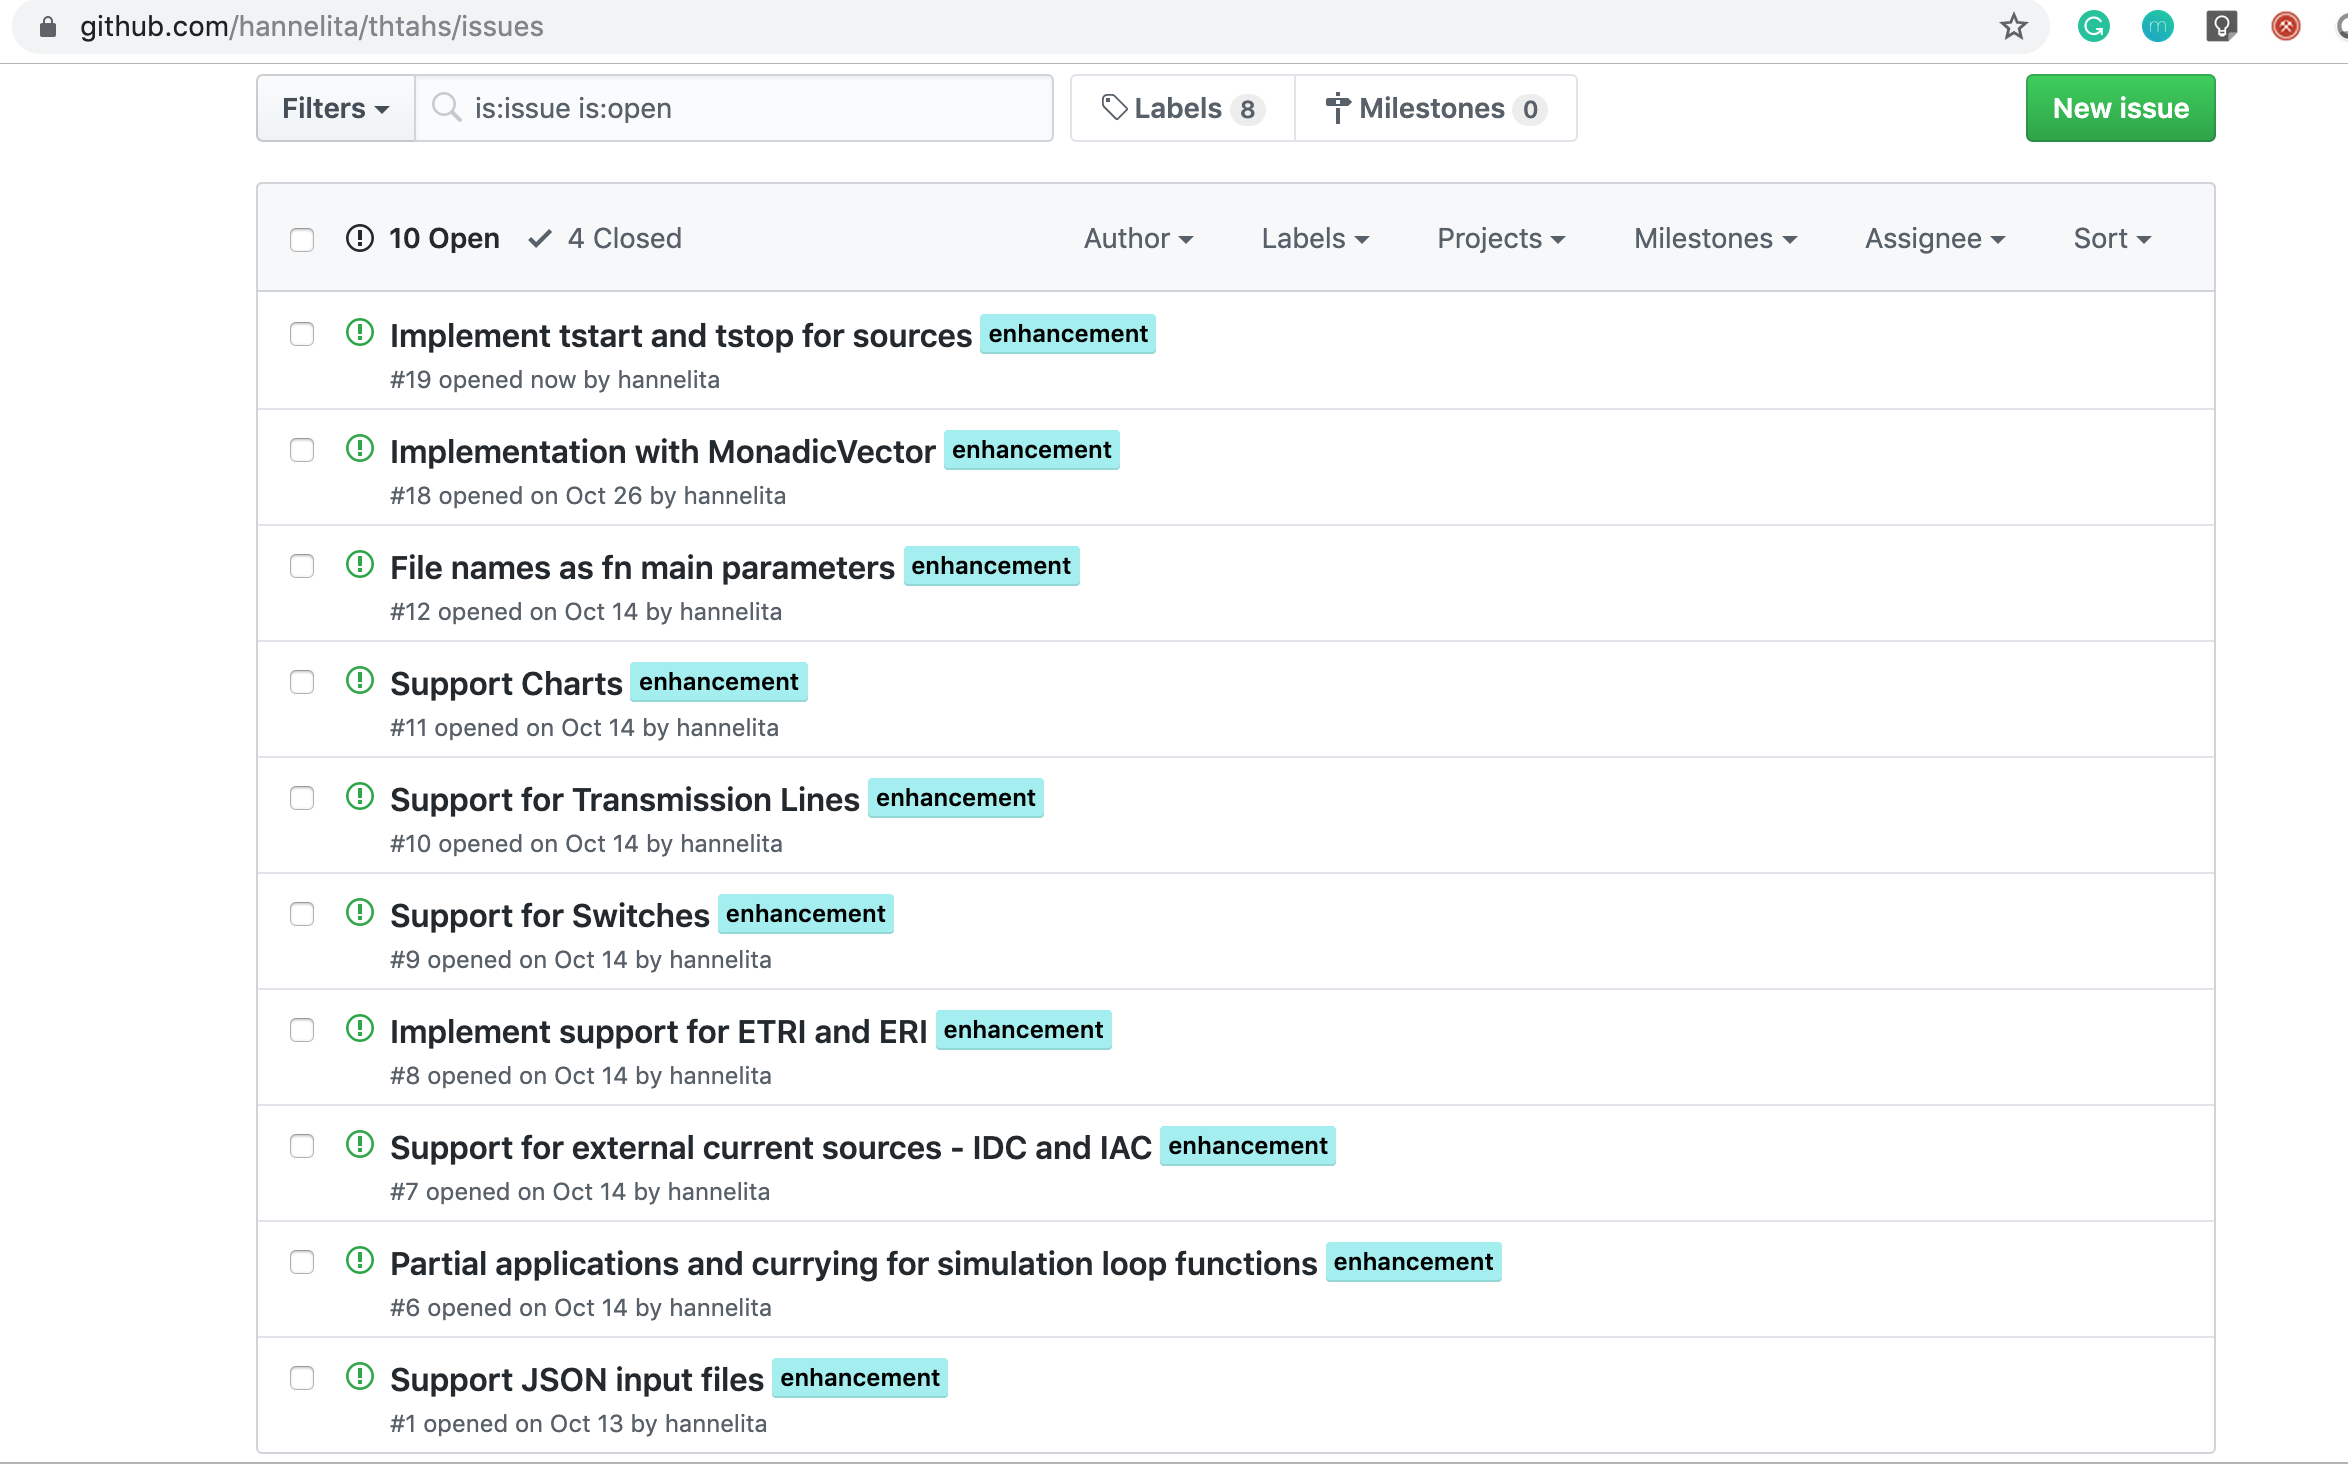
\includegraphics[width=0.7\textwidth]{img/featuresgithub.png}
   \caption{Issue tracker on Github for the Haskell ETR-P project.}
   \label{fig:featuresgithub}
\end{figure}

\section{Final thoughts}

This work was deeply related with abstraction and types. In fact, abstracting the code and abstracting the engineering model of the nodal equations were both joint into the implementation of this Haskell code. By finding ways to abstract the code, it is possible to find more concise ways to represent and explain the physical model. From the equation $[G][V] = [Ih]$ in chapter \ref{ch:etr} to the main Haskell function signature in chapter \ref{implhs} \lstinline!thtaSimulation :: Vector ComponentData -> SimulationData -> SimulationResults! a lot of abstration was built. Are these two representations equivalent? This work does not provide any proof of it. But it provides the reader with the formal and technical tools to give an intuition on how to investigate this matter. 



